In questo capitolo si vuole presentare il quadro attuale della situazione attorno ai sistemi blockchain. Nuove tecnologie sono sviluppate continuamente, perciò dopo una breve panoramica sui progetti più interessanti già in stadio avanzato di sviluppo si illustreranno le sfide e gli ambiti di ricerca più ferventi, fino ad arrivare ad elencare alcune delle applicazioni che potrebbero conseguire dai risultati di tali ricerche.

\section{Innovazioni vicine}
    Nel 2017 si è verificata una crescita rapidissima di Bitcoin, tale da portare l'argomento al di fuori degli ambiti specialistici e farlo diventare un vero e proprio fenomeno di massa.
    \begin{figure}[ht]
        \centering
        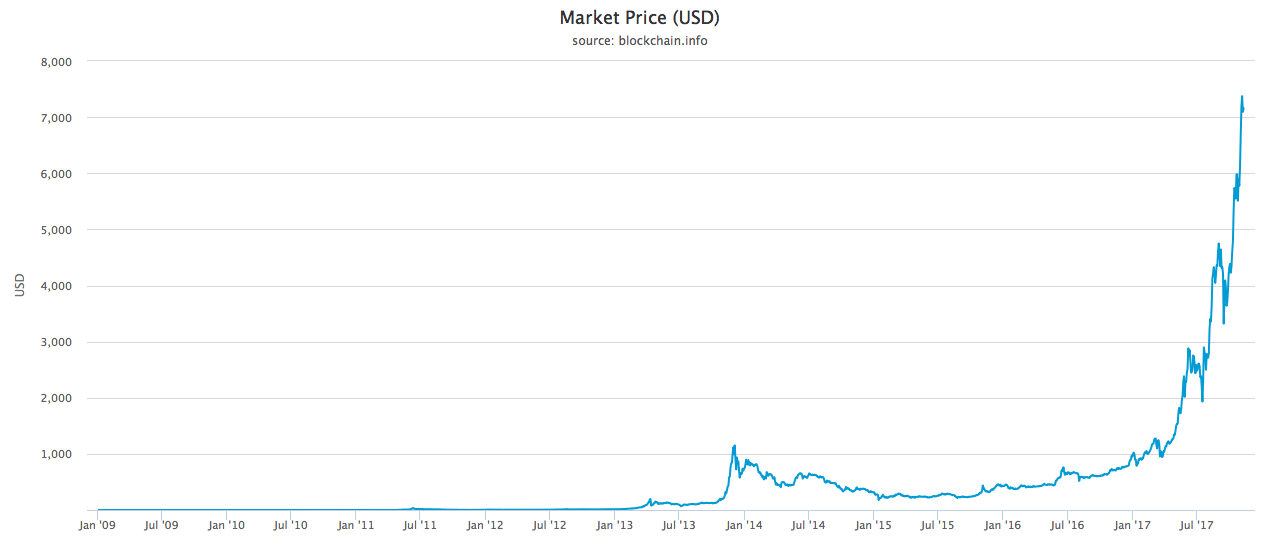
\includegraphics[width=\textwidth]{bitcoin-price.png}
        \caption[Valore di mercato di Bitcoin nel 2017]{Crescita del valore di mercato di Bitcoin nel 2017.}
        \label{fig:bitcoin_price}
    \end{figure}
    Dietro a Bitcoin si è sviluppata un'enorme quantità di applicazioni e sperimentazioni che riguardano blockchain, alcune delle quali hanno raggiunto ormai una certa stabilità. Molte di queste riguardano l'ambito economico e prendono il nome di \emph{criptomonete}, altre invece si basano sulla blockchain per costruire sistemi più complessi.

    \paragraph{Il crollo delle criptovalute} ~ \\
    Non tutti i progetti avviati negli ultimi anni vanno però a buon fine.
    Le dichiarazioni del governo sudcoreano prospettanti un possibile blocco delle criptovalute, avvenute a metà gennaio, hanno inaugurato un periodo difficoltoso per il mercato delle monete basate su blockchain. Prendendo come riferimento Bitcoin, che si mantiene al primo posto per quanto riguarda il valore di mercato e pertanto riflette piuttosto bene l'andamento generale, dopo aver raggiunto il picco di circa 19'500 dollari a metà dicembre ha visto il suo valore crollare a poco meno di 7'000 dollari, con giornate particolarmente critiche che hanno registrato svalutazioni di oltre il 10\% nell'arco di 24 ore.

        \begin{figure}[ht]
            \centering
            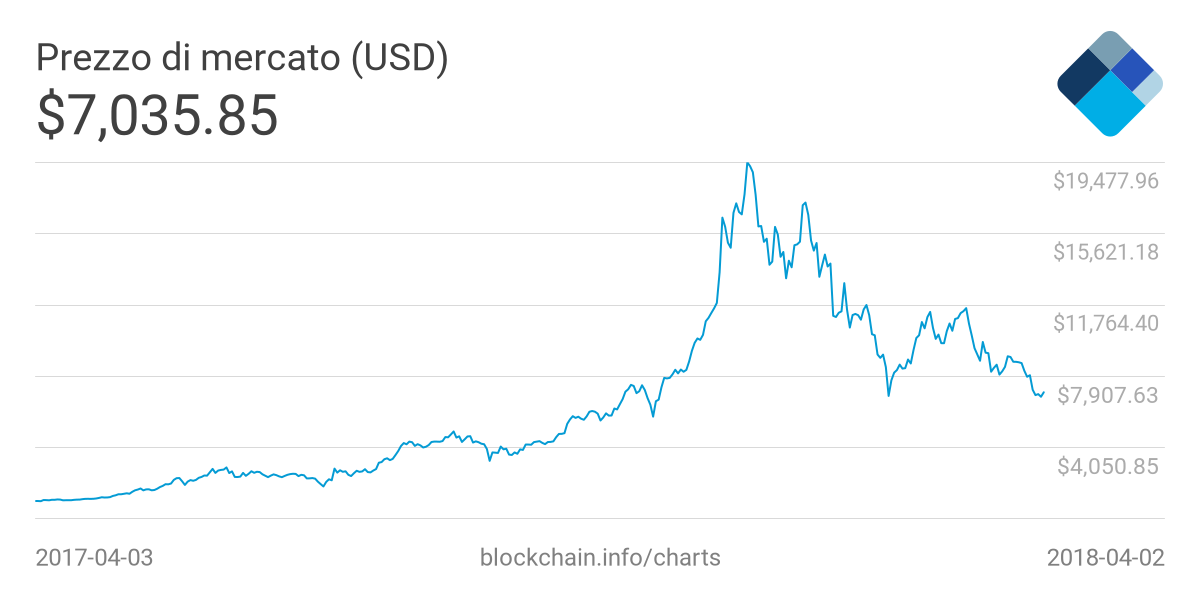
\includegraphics[width=\textwidth]{bitcoin-price-update.png}
            \caption[Valore di Bitcoin nell'ultimo anno]{Valore di Bitcoin nell'ultimo anno.}
            \label{fig:bitcoin-price-update}
        \end{figure}

    L'intero ecosistema che ruota attorno alla tecnologia blockchain è stato condizionato dalla disillusione portata dal crollo delle criptovalute. Molti progetti si sono arenati e, in generale, ci si sta rendendo conto delle difficoltà di sviluppo e mantenimento di tali sistemi \cite{blockchain_delusion}. Questo non ha fermato l'avanzamento di altri gruppi di lavoro, i cui prodotti hanno raggiunto la stabilità necessaria per proporsi come \emph{stabili}.

    Di seguito si riportano alcune soluzioni tra le più affermate basate su tecnologia blockchain disponibili. L'elenco non è esaustivo, poiché lo scenario è estremamente mutevole, ma mira a fornire una visione di insieme che possa essere una buona base per ricerche ulteriori.
    
    \subsection{Criptomonete}
        \begin{itemize}
            \item \textbf{Ripple}: è il più famoso sistema di scambio di valuta basato su blockchain permissioned, adottato tra gli altri da MUFG, RBC, Santander, Unicredit, BBVA \url(https://ripple.com/);
            \item \textbf{Litecoin}: è una criptomoneta molto simile a Bitcoin da cui differisce per alcune caratteristiche chiave, su tutte il tempo necessario all'elaborazione di un blocco (2 minuti e mezzo contro i 10 minuti di Bitcoin) e il sistema di consenso. Litecoin infatti usa \emph{scrypt} per la sua proof-of-work, una funzione gravosa sulla memoria piuttosto che sul processore che punta a evita il predominio delle server farm con hardware dedicato che controllano le operazioni di mining di Bitcoin;
            \item \textbf{Peercoin}: è una criptomoneta alternativa che adotta un algoritmo di consenso ibrido tra proof-of-work e proof-of-stake, allo scopo di portare un'alternativa solida all'enorme consumo energetico di Bitcoin;
            \item \textbf{Monero}: fork di Bitcoin che utilizza CryptoNote, un protocollo basato sulla Ring Signature orientato a rafforzare l'anonimato nella blockchain;
            \item \textbf{ZCash e ZCoin}: come Monero si pongono l'obiettivo di garantire la privacy in un sistema blockchain, usano algoritmi di tipo zero-knowledge sebbene con piccole differenze tra di loro \cite{zcoin_vs_zcash};
        \end{itemize}
        Un'altra applicazione interessante a livello economico è quella legata all'uso di criptomonete per il crowd-funding. Questa trova una semplice implementazione direttamente in Bitcoin attraverso l'uso di quello che si chiama \emph{assurance contract}. Si tratta di una transazione con un singolo output rappresentante l'obiettivo del finanziamento, a cui si unisce poi ciascun volontario partecipante tramite hash di tipo \emph{SIGHASH\_ALL} e \emph{SIGHASH\_ANYONECANPAY}, che permettono di modificare gli input di transazione ma non gli output (si rimanda alla documentazione ufficiale per approfondimento). La transazione può essere registrata in blockchain, e quindi essere effettiva, solo quando il valore di output è coperto da corrispondente valore in input, ovvero al raggiungimento dell'obiettivo della campagna di crowd-funding.
     
    \subsection{Non-Criptomonete} \label{sec:non-crypto}
        \begin{itemize}
            \item \textbf{Ethereum}: si tratta del principale sistema basato su blockchain dopo Bitcoin. Il suo scopo è quello di permettere la creazione di applicazioni decentralizzate, che vengono eseguite come smart contract distribuiti tra i peer che partecipano alla rete. È il primo sistema blockchain ad aver introdotto un linguaggio Turing-completo (\emph{Solidity}) e il concetto di macchina virtuale su blockchain, nel 2013. Si basa su una propria moneta virtuale che viene utilizzata per ``alimentare" le applicazioni distribuite (in ambito Ethereum si parla di \emph{gas}, abbreviazione di \emph{gasoline}). Questa si chiama \emph{Ether}, e al momento si trova saldamente al secondo posto come market cap dietro a Bitcoin.

            La rete di Ethereum si è recentemente trovata interessata da un considerevole aumento di carico, con il picco massimo nel mese di gennaio, dovuto alla diffusione dei \emph{Crypto Kitties}. Si tratta di animaletti digitali, simili ai più datati Tamagochi, che vivono e si riproducono nella blockchain di Ethereum alimentando un correlato mercato di collezionisti. Il traffico da loro generato è arrivato a rappresentare oltre il 20\% del traffico totale di Ethereum, il quale si è mostrata capace di affrontare l'impennata di transazioni adeguatamente seppure con una risposta iniziale piuttosto lenta che ha fatto temere per il congestionamento del sistema.

            \begin{figure}[ht]
                \centering
                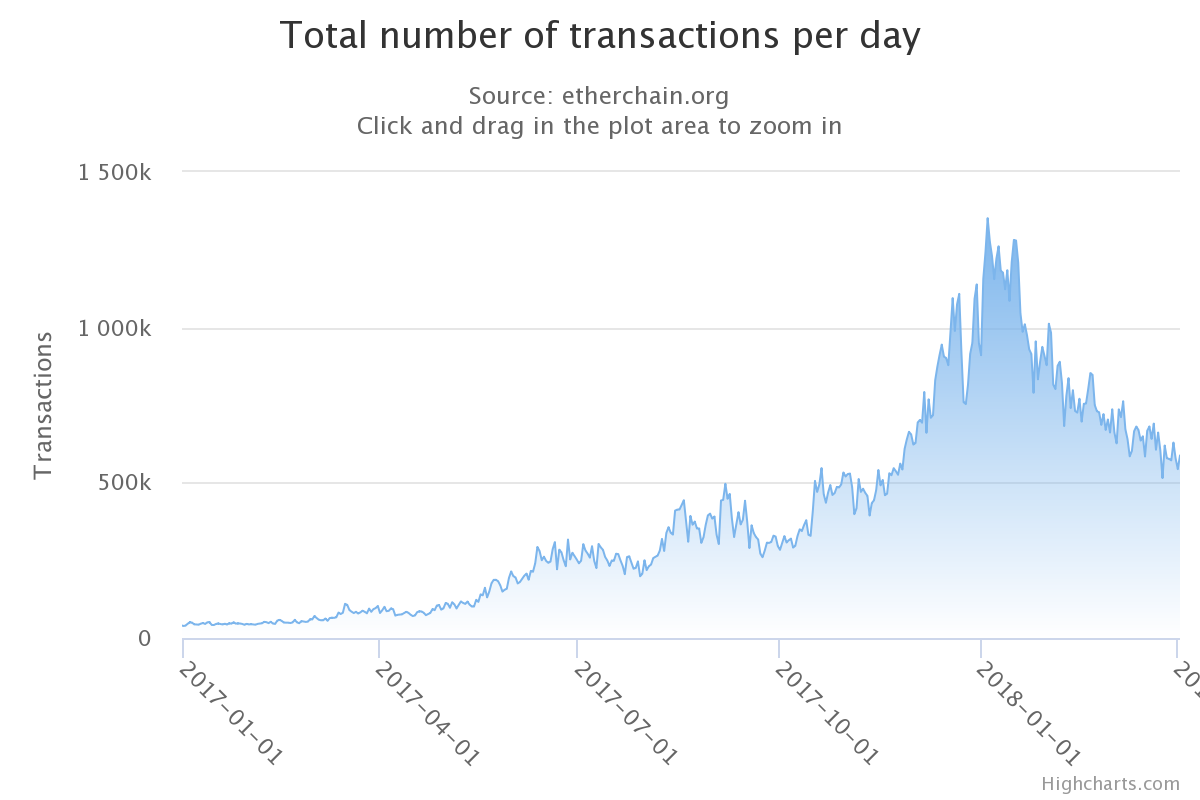
\includegraphics[width=\textwidth]{ethereum-load.png}
                \caption[Numero di transazioni giornaliere su Ethereum]{Numero di transazioni giornaliere su Ethereum.}
                \label{fig:ethereum-load}
            \end{figure}

            \item \textbf{Hyperledger Sawtooth}: Sawtooth è il framework del progetto Hyperledger a cui contribuisce Intel. Riprende l'idea di framework modulare propria di Fabric, ma ne rappresenta una versione maggiormente decentralizzata e indipendente da un ordering service sfruttando un particolare algoritmo di consenso di default, detto Proof of Elapsed Time (PoET), che permette un funzionamento simile a quello della rete Bitcoin prescindendo dai problemi di consumo energetico in precedenza descritti. Hyperledger Sawtooth punta soprattutto alla versatilità supportando sia configurazioni di tipo permissioned che di tipo permissionless, unico progetto Hyperledger a farlo. Recentemente è uscita la versione 1.0.1, che ne sancisce la raggiunta stabilità;

            \item \textbf{Hyperledger Iroha}: Iroha è un framework blockchain a cui contribuiscono Soramitsu, Hitachi, NTT Data e Colu. Hyperledger Iroha è progettato per essere semplice da integrare in progetti di infrastrutture basate su blockchain. Punta soprattutto allo sviluppo di applicazioni mobile, fornendo librerie client per Android e iOS. Ispirandosi a Hyperledger Fabric, Hyperledger Iroha cerca di fare da complemento ad Hyperledger Fabric e Hyperledger Sawtooth, fornendo nel contempo un ambiente di sviluppo per i programmatori C++ interessati a contribuire al progetto Hyperledger;

            \item \textbf{Hyperledger Indy}: è un sistema progettato per la gestione di identità digitali. Si avvale dei contributi della Sovrin Foundation ed è qui riportato come scenario futuro interessante: la riuscita di un progetto di questo tipo porterebbe un'accelerazione a tutti quei sistemi blockchain che necessitato di autenticazione utente, operazione finora relegata off-chain e a responsabilità di un garante. L'inserimento di Indy tra i progetti Hyperledger è sufficiente per richiamare l'attenzione sui suoi sviluppi futuri, sperando che presto raggiunga abbastanza stabilità da poterci basare altri servizi. Una notevole spinta in questo senso è quella data dai molteplici tentativi di standardizzazione, oggetto dei lavori congiunti di \emph{W3C} e della community \emph{Rebooting The Web Of Trust} \cite{rebooting_web_of_trust};

            \item \textbf{Quorum}: creata da JPMorgan, Quorum è di fatto un fork della blockchain pubblica di Ethereum che usa un algoritmo di consenso basato su votazione per fornire una piattaforma orientata all'uso enterprise di smart contract. La privacy dei dati è raggiunta nella rete di Quorum esponendoli sulla base delle necessità effettive del nodo;

            \item \textbf{OpenTimestamps}: servizio che mira a diventare uno standard per il timestamping via blockchain. Concatena hash crittografici dei dati di cui gli utenti richiedono il timestamping e ne registra il risultato in una transazione bitcoin, rendendolo quindi pubblico e immutabile;

            \item \textbf{Namecoin}: servizio basato su blockchain che si propone di potenziare decentralizzazione, sicurezza, resistenza alla censura, privacy e velocità di componenti alcune dell'infrastruttura di Internet come i DNS;

            \item \textbf{Everledger}: una nicchia promettente riguarda i sistemi ad-hoc con utilizzo ben preciso. Ne è un esempio Everledger, che si propone di tracciare e gestire storia e possesso di beni di lusso come i diamanti;

            \item \textbf{Filament}: la natura distribuita di blockchain la rende ideale per implementazione di applicazioni IoT che richiedano un adeguato livello di sicurezza. Lavora in questo ambito Filament, startup nata recentemente, nel 2017, che si pone come obiettivo la gestione di reti wireless sicure in ambito IoT;

            \item \textbf{Blockchain a livello enterprise}: per la creazione di applicazioni aziendali basate su blockchain è necessario appoggiarsi ad opportuni framework. Questi devono rispettare requisiti imprescindibili per l'ambito business, tra cui fornire opportuna documentazione, supporto tecnico e rendere agevoli le operazioni di testing, integrazione, controlli di sicurezza. Esempi di piattaforme simili in sviluppo sono Hyperledger, Bloq, Chain, sebbene ciascuno di questi soffra al momento di poca stabilità dovuta alla loro ancora recente nascita;
            
            \item \textbf{Hawk}: è un sistema di smart contract che affronta il problema della poca privacy nelle transazioni delle blockchain più diffuse. Hawk fornisce uno strumento per la generazione di un ``protocollo crittografico efficiente in cui le controparti del contratto interagiscono con la blockchain usando primitive crittografiche come gli algoritmi \emph{zero-knowledge proof}." \cite{hawk};
        \end{itemize}

\section{Sfide e ambiti di ricerca}

    \subsection{Efficienza e scalabilità}
        Sono essenzialmente due gli obiettivi di ricerca per la soluzione ai problemi di efficienza e scalabilità, ovvero:
        \begin{itemize}
            \item Algoritmi di consenso;
            \item Problemi crittografici nuovi.
        \end{itemize}
        Il problema della scalabilità dei sistemi blockchain è molto dipendente dall'algoritmo di consenso implementato. Quelli ad oggi adottati su larga scala sono basati su proof-of-work, che paradossalmente basa la sua sicurezza sulla sua assoluta inefficienza. Inoltre, la storia di Bitcoin mostra come sia inefficace nel mantenere equilibrata la competizione tra i miner, portando un accentramento delle capacità di gestione della rete nelle mani di server farm dedicate. Ethereum migliora questo aspetto attraverso un algoritmo simile, ma in cui ha meno vantaggi investire in hardware dedicato. Tuttavia la ricerca ad un algoritmo che permetta l'effettiva ``democratizzazione'' del mining è ancora apertissima, accompagnata da quella su problemi crittografici meno parallelizzabili su cui basare ulteriori varianti degli algoritmi proof-of-work.
        
    \subsection{Standardizzazione e interoperabilità}
        Blockchain non è ancora una tecnologia sufficientemente matura da permettere una piena ed agevole integrazione con i sistemi esistenti. Emettere degli standard adeguati aiuterà a migliorare l'integrazione dei sistemi blockchain tanto fra di loro quanto con l'infrastruttura circostante. \\
        Dal punto di vista applicativo lo sviluppo di framework come Hyperledger aiuta a creare una base solida e delle sottostrutture chiare per la progettazione di reti distribuite interoperanti, e maggiore sarà il numero di utenti che abbracceranno soluzioni di questo tipo minori saranno le differenze critiche tra sistema e sistema permettendo adattamenti più agevoli. D'altra parte, è necessario che tali piattaforme si sviluppino e allarghino la gamma di scenari modellabili venendo incontro alle necessità di gruppi di utenti sempre più grandi ed eterogenei. \\
        Dal punto di vista normativo invece si sono visti passi in avanti con la creazione nel 2016 del comitato tecnico ISO/TC 307 ``blockchain and distributed ledger technologies", che sta sviluppando il primo standard ISO ufficiale sull'argomento.

    \subsection{Privacy}
        Si possono distinguere due punti chiave in cui si sta lavorando per migliorare l'aspetto relativo alla privacy su blockchain. In primo luogo, l'uso di pseudonimi non può certo considerarsi un modo sicuro per nascondere l'identità che si cela dietro questi. In secondo luogo, in determinati casi è desiderabile garantire la riservatezza di alcuni dati salvati in catena, magari restringendone l'accesso solo a determinati utenti. Si riportano nel seguito alcune soluzioni a questi problemi.
        
        \subsubsection{Mixer}
            Prendono il nome di \emph{mixer} tutte quelle tecnologie applicabili ai sistemi basati su token che permettono di offuscare mittente e destinatario delle transazioni senza intervenire direttamente sul protocollo. \\
            Esempi notevoli sono \emph{CoinJoin} e \emph{CoinSwap}. \\
            \begin{itemize}
                \item In CoinJoin, più utenti concordano di ``mescolare" una certa quantità di valuta e creano una singola transazione multi-input e multi-output, mescolando letteralmente i coin in loro possesso. Ciò permette di confondere la maggior parte delle strategie di analisi del traffico, poiché presuppongono tipicamente che gli indirizzi in input per ogni transazione appartengano allo stesso utente. Come altri servizi di mixing, non rende impossibile rompere l'anonimato degli indirizzi ma lo rende più difficoltoso.
                \item CoinSwap sfrutta invece un utente terzo che faccia da intermediario tra le controparti della transazione. Per garantire che l'intermediario rispetti l'accordo e non imbrogli il sistema, CoinSwap fa uso di transazioni bloccate, che possono essere sbloccate solo conoscendo la controimmagine di un dato hash (\emph{hashlocked transaction}) e che sono pubblicate in chain solamente nel caso l'intermediario non rispetti gli accordi. La pubblicazione delle hashlocked transaction rompe l'anonimizzazione creata ma impedisce azioni malevole.
                \begin{figure}
                    \centering
                    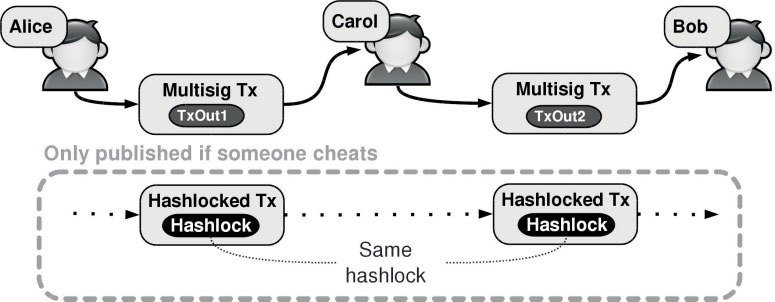
\includegraphics[width=0.8\textwidth]{coinswap.jpg}
                    \caption[Transazione CoinSwap]{Transazione CoinSwap.}
                    \label{fig:coinswap}
                \end{figure}
            \end{itemize}
        
        \subsubsection{Condivisione selettiva di dati sensibili}
            Un possibile compromesso per tutelare la privacy dei dati condivisi riguarda la suddivisione del sistema in sotto-catene, in modo che ciascuna transazione sia condivisa non con la totalità dei nodi, ma solamente tra le due controparti ed un ristretto insieme di controllori. Pur apprezzabile per quanto riguarda privacy e scalabilità, questo approccio va a ridurre sensibilmente la sicurezza dell'intero sistema. Non esiste più infatti una singola catena di transazioni concordate, e l'immutabilità del registro è tanto più debole quanti meno sono i nodi a conoscenza della transazione.
            
        \subsubsection{Frammentazione dei dati}
            Si potrebbero gestire dati criptati su blockchain affidandone la manipolazione a diversi partecipanti in maniera frammentaria. Le operazioni sono suddivise in frammenti non riconoscibili e distribuite in modo che ciascun nodo non abbia sufficienti informazioni da ricostruire il contesto da cui i dati provengono. Un esempio di protocollo che permette di ottenere un simile risultato è quello adottato dal sistema Enigma, sviluppato dal MIT \cite{enigma}.
            
        \subsubsection{Algoritmi zero-knowledge}
            Uno degli argomenti più dibattuti in crittografia negli ultimi anni sono le \emph{zero-knowledge proof}. Si tratta di funzioni matematiche che possono essere eseguite su dati criptati in maniera che il loro risultato possa essere validato senza alcuna esposizione di dati non criptati. Acquistano un interesse particolare soprattutto pensando a sistemi basati su smart contract: potenzialmente permettono a diversi nodi di lavorare su uno smart contract senza che vengano loro rivelati i dati su cui stanno operando. Un primo esempio di applicazione di algoritmi zero-knowledge è zCash, che si basa su zk-SNARK \cite{zkSNARK}.

\section{Cosa si potrà fare}
	A raggiunta maturità tecnologica, blockchain potrà avere un ruolo chiave nella realizzazione di molteplici use case. Di seguito ne propongo alcuni relativamente vicini ed implementabili in un prossimo futuro, magari attraverso una collaborazione tra Infocamere e altre grandi aziende legate alla pubblica amministrazione.
		
    \subsubsection{Reti IoT sicure}
        	In quanto sistema distribuito e decentralizzato, blockchain si propone come tassello fondamentale nella creazione di reti IoT sicure e certificate. Lo use case preso ad esempio da Hyperledger Sawtooth per illustrare sue potenzialità è proprio l'applicazione di blockchain ad una rete di sensori che traccino e certifichino la catena di produzione di beni deperibili come il pesce. Non è difficile immaginare molteplici applicazioni analoghe, in particolare riguardanti la certificazione di strumenti di misurazione di precisione o apparecchi di controllo quali i cronotachigrafi;
        	
        \subsubsection{Digital Identity}
        	La creazione di un sistema di identità digitale è già stata presentata come \emph{work in progress} da parte di fondazioni come la Sovrin. Se una gestione completamente autonoma della propria identità digitale è un progetto a lungo termine, potrebbe non esserlo invece l'applicazione di blockchain a sistemi già in essere come lo SPID. Il livello di sicurezza garantito sarebbe sufficiente ad integrare questi sistemi con una serie di funzionalità interessanti, tra cui ad esempio un sistema di firma digitale estremamente più \emph{personale} e flessibile rispetto a quello di cui si può disporre oggi.
        	
        	La firma digitale richiede infatti una serie di precauzioni considerevole. Immaginiamo a titolo esemplificativo di firmare un documento a valore legale utilizzando un qualsiasi sistema a chiave asimmetrica: ci si aspetta che questo documento possa rimanere disponibile per anni, e che la firma di ciascuno non sia usa e getta ma venga riutilizzata per firmare ogni documento. Ora, violare questa firma comporterebbe il decadimento della validità di tutti i documenti passati, presenti e futuri marcati attraverso di essa dal momento che questi potrebbero essere retrodatati da parte del ladro. Potrebbe non essere sufficiente nemmeno affidarsi a servizi di timestamping: se fosse proprio la chiave privata del server di timestamping ad essere trafugata, tutti i documenti precedenti alla compromissione della firma sarebbero completamente invalidati.
        	
        	\begin{figure}[ht]
        		\centering
        		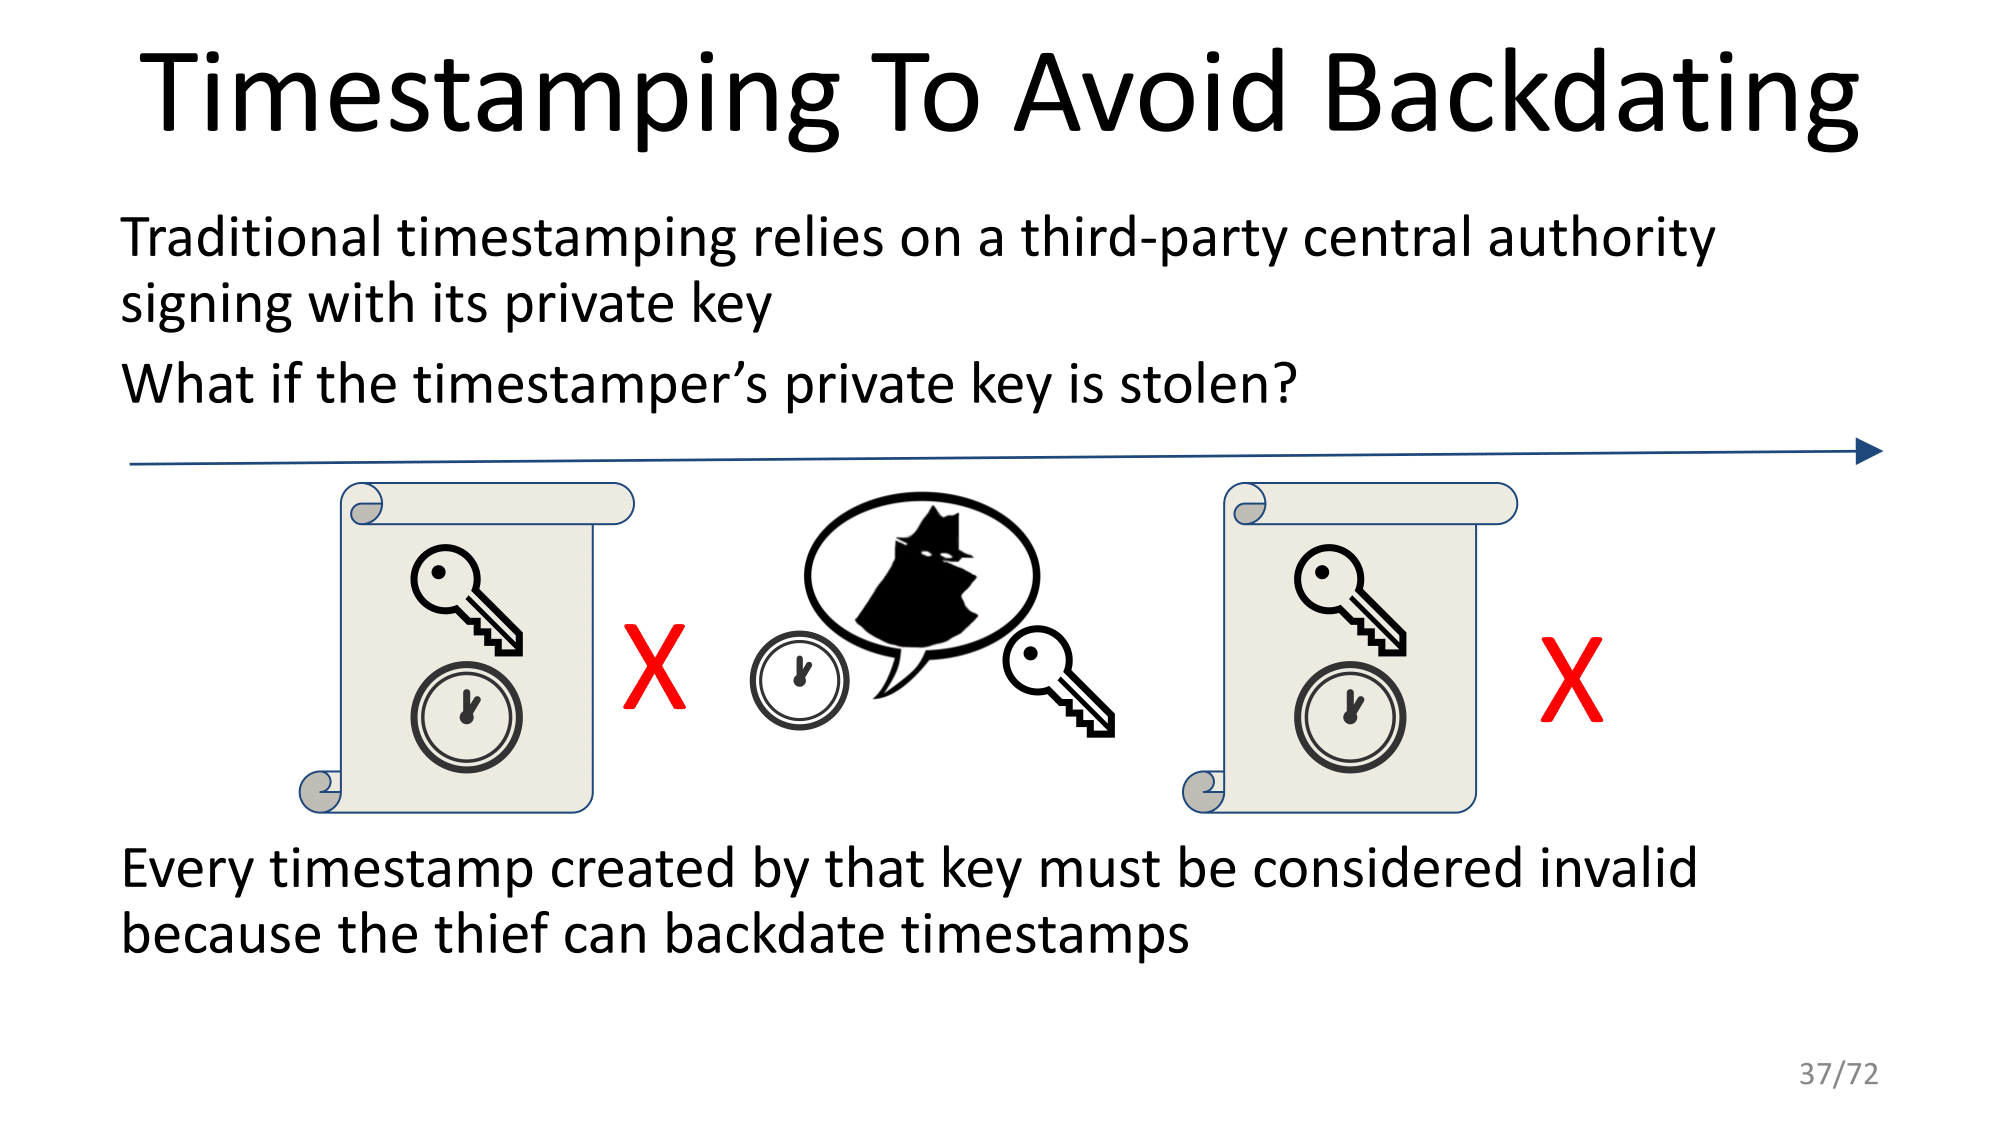
\includegraphics[width=\textwidth]{key-1.png}
        		\caption[Furto della chiave privata]{Furto della chiave privata. \cite{ametrano_signature}}
        		\label{fig:key-1}
        	\end{figure}
        	
   			Fornire un sistema di firma digitale su blockchain che permettesse funzionalità di gestione della firma quali emissione della chiave pubblica, pubblicazione del certificato di revoca e timestamping dei documenti firmati, potrebbe rappresentare una soluzione efficace ed efficiente ai problemi sopra esposti. Sfrutterebbe l'immutabilità e la sicurezza di blockchain per impedire la falsificazione del timestamp, e se legato ad un sistema ``ufficiale" di identità digitale potrebbe avere valore legale pur rimanendo personale nella gestione.
   			
   		\subsubsection{Controlli sull'immigrazione}
   			Un altro ambito legato all'identità digitale che può rappresentare un ottimo use case per blockchain è la gestione dell'identità dei rifugiati. Sarebbe possibile non solo condividere i dati necessari all'identificazione, ma anche spostare tutta la gestione degli aiuti economici on-chain prescindendo quindi dalla moltitudine di organizzazioni che al momento fanno da intermediari, senza gravare eccessivamente sull'apparato statale. Inoltre, la trasparenza di blockchain si coniuga molto bene con le necessità di controllo da parte di più enti su questi dati, e alla condivisione degli stessi anche tra più stati nel caso poi il rifugiato continui il proprio viaggio verso altri paesi.
   			
   		\subsubsection{Gestione di proprietà}
   			Bitcoin è nato per modellare una sorta di oro digitale. In maniera molto simile, è possibile implementare un sistema blockchain che gestisca il possesso e il commercio di una generica proprietà. Ciascun \emph{Digital Asset} vivrebbe on-chain e potrebbe essere trasferito di proprietario in proprietario senza bisogno della certificazione di un notaio o di altro ente esterno. Un sistema di smart contract potrebbe garantire che norme su controlli periodici obbligatori o pagamento di tasse come il bollo auto venissero rispettate correttamente, e l'intera storia dell'asset sarebbe tracciata e registrata con una trasparenza finora impensabile.
   			
   			Un simile sistema semplificherebbe in maniera notevole la gestione dei DRM (\emph{Digital Rights Management}) permettendo a chiunque di registrare la proprietà individuale di un opera che possa essere digitalizzata in qualche modo creando a tutti gli effetti il corrispondente asset e assegnandone a se la proprietà. Ciò aprirebbe ad una razionalizzazione del sistema di riconoscimento dei compensi derivati dai diritti di autore, che potrebbe essere spostata on-chain e automatizzata.
